\documentclass[11pt]{article}

% Packages
\usepackage[margin=1in]{geometry}
\usepackage{amsmath,amssymb,amsthm}
\usepackage{natbib}
\usepackage{graphicx}
\usepackage{booktabs}
\usepackage{xcolor}
\usepackage{hyperref}
\usepackage{cleveref}
\usepackage{tikz}
\usetikzlibrary{arrows.meta, positioning, calc, fit, backgrounds, shapes.geometric, decorations.pathreplacing}

% Custom commands

\theoremstyle{definition}
\newtheorem{assumption}{Assumption}
\newtheorem{decision}{Decision}

\title{Buttressing-Mediated State-Variable Model for\\
  WAIS Mass Loss Projections\\[6pt]
  \large Ar\^{e}te / Hierarchical SLR Framework --- Working Document}

\author{Working Draft}
\date{2026-03-04}

\begin{document}
\maketitle

\begin{abstract}
This document develops a causal evolution equation for West Antarctic Ice Sheet (WAIS) mass loss in which ice-shelf buttressing is the central latent state variable mediating between external forcing and glacier dynamics.  The model replaces the direct forcing-to-rate coupling of the previous Approach~A formulation with a two-layer causal structure: forcing drives buttressing evolution, and buttressing loss drives glacier acceleration.  This correction to the causal graph enables clean representation of interventions that target buttressing directly (seabed-anchored curtains), interventions that target basal conditions (Kamb-style glacier stagnation via subglacial water/heat manipulation), and interventions that modify forcing (MCB, SAI).  The document derives the buttressing--flux coupling exponent from three theoretical frameworks (Pegler, Schoof, Haseloff), develops a structural failure parameterisation calibrated against remote-sensing-derived tensile strength estimates, and generalises the basal resistance term to include effective pressure and sliding-law dependence.
\end{abstract}

\tableofcontents
\newpage

% ====================================================================
\section{Causal Structure}
\label{sec:causal}
% ====================================================================

\subsection{Why the Previous Model Was Causally Wrong}

The previous Approach~A evolution equation coupled ocean thermal forcing directly to the rate of change of the mass-loss rate:
\begin{equation}
  \frac{dr}{dt} = \alpha \cdot [T_{\text{ocean}}(t) - T^{*}]_+ + \gamma_{\text{eff}}(r) \cdot r(t) + \epsilon(t).
  \label{eq:old_4A}
\end{equation}
This conflates two distinct physical links in the causal chain.  The actual mechanism is:
\begin{equation}
  T_{\text{ocean}}(t) \;\longrightarrow\; \text{shelf thinning} \;\longrightarrow\; \text{buttressing loss} \;\longrightarrow\; \text{stress change at GL} \;\longrightarrow\; \text{acceleration}.
  \label{eq:causal_chain}
\end{equation}
Collapsing this chain into a single sensitivity parameter $\alpha$ has three consequences that are fatal for the intended use of the framework:

\begin{enumerate}
  \item \textbf{Intervention channel is wrong.}  Thwaites stabilisation via seabed-anchored curtains is a do-intervention on buttressing, not on $T_{\text{ocean}}$.  Basal interventions are downstream of buttressing in the flux equation.  Neither has a clean representation in \cref{eq:old_4A}.

  \item \textbf{Committed dynamics are misrepresented.}  Structural damage to ice shelves (calving, shear-margin rupture, loss of pinning-point contact) is effectively irreversible on projection timescales.  If $T_{\text{ocean}}$ returns below $T^{*}$, the forced-acceleration term in \cref{eq:old_4A} vanishes, but the physical buttressing deficit persists.  The model lacks memory of structural state.

  \item \textbf{The flow-law exponent $n$ has no natural entry point.}  Martin et al.\ (in review) show that higher $n$ reduces buttressing effectiveness because shear-thinning concentrates strain and weakens the shelf's capacity to transmit lateral stresses.  This effect enters through the buttressing evolution, not through the mass-loss rate equation.
\end{enumerate}

\subsection{Directed Acyclic Graph}

The corrected causal structure for a single basin $i$ is:

\begin{center}
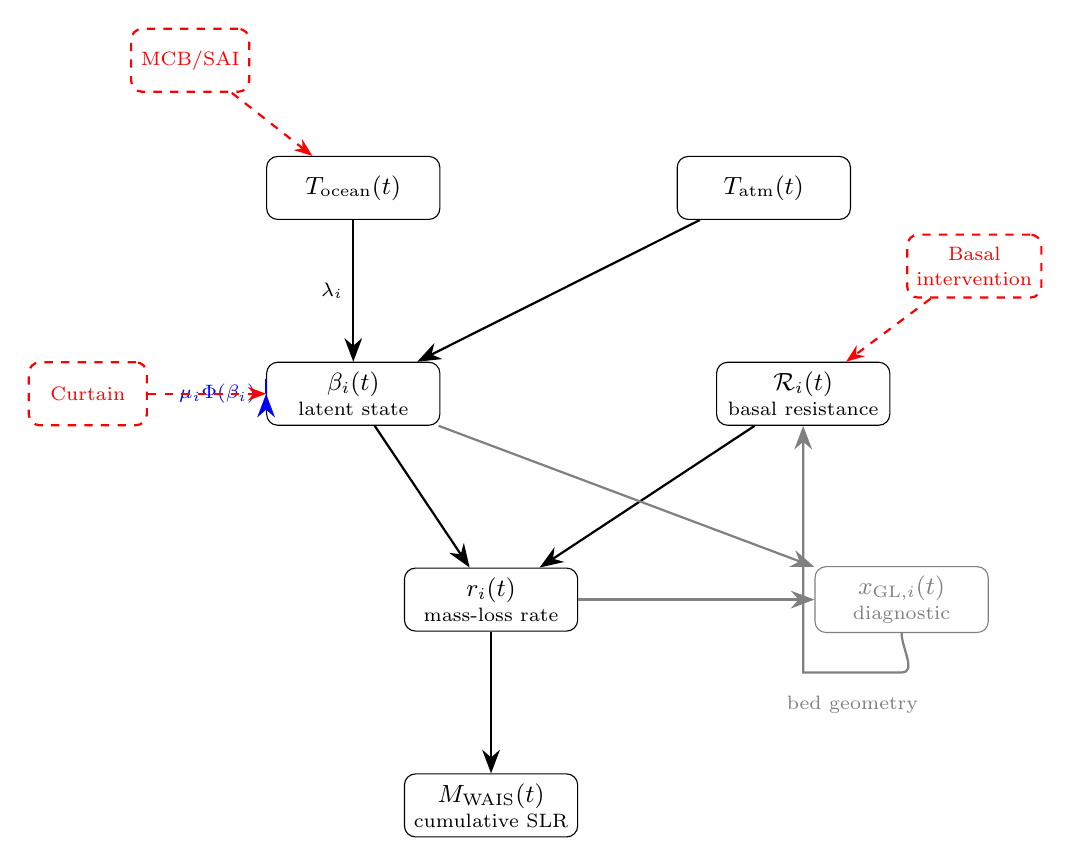
\begin{tikzpicture}[
  node distance=1.8cm and 2.5cm,
  every node/.style={draw, rounded corners, minimum width=2.2cm, minimum height=0.8cm, align=center, font=\small},
  arrow/.style={-{Stealth[length=3mm]}, thick},
  intervention/.style={draw, dashed, red, thick, rounded corners},
  ]

  % Forcing nodes
  \node (Tocean) {$T_{\text{ocean}}(t)$};
  \node[right=3cm of Tocean] (Tatm) {$T_{\text{atm}}(t)$};

  % Buttressing
  \node[below=of Tocean] (beta) {$\beta_i(t)$\\[-2pt]\scriptsize latent state};

  % Basal resistance
  \node[right=3.5cm of beta] (Rbasal) {$\mathcal{R}_i(t)$\\[-2pt]\scriptsize basal resistance};

  % Rate
  \node[below=of beta, xshift=1.75cm] (r) {$r_i(t)$\\[-2pt]\scriptsize mass-loss rate};

  % Cumulative
  \node[below=of r] (M) {$M_{\text{WAIS}}(t)$\\[-2pt]\scriptsize cumulative SLR};

  % GL position (diagnostic)
  \node[right=3cm of r, draw=gray, text=gray] (xGL) {$x_{\text{GL},i}(t)$\\[-2pt]\scriptsize diagnostic};

  % Arrows
  \draw[arrow] (Tocean) -- node[left, draw=none, font=\scriptsize, minimum width=0] {$\lambda_i$} (beta);
  \draw[arrow] (Tatm) -- (beta);
  \draw[arrow] (beta) -- (r);
  \draw[arrow] (Rbasal) -- (r);
  \draw[arrow] (r) -- (M);
  \draw[arrow, gray] (r) -- (xGL);
  \draw[arrow, gray] (beta) -- (xGL);

  % Self-loop for structural failure
  \draw[arrow, blue] (beta.west) to[out=150,in=210,looseness=4] node[left, draw=none, font=\scriptsize, text=blue, minimum width=0] {$\mu_i \Phi(\beta_i)$} (beta.west);

  % Feedback from GL to basal resistance
  \draw[arrow, gray] (xGL.south) to[out=-90,in=0] ++(0,-0.5) -| node[near start, below, draw=none, font=\scriptsize, text=gray, minimum width=0] {bed geometry} (Rbasal.south);

  % Intervention nodes
  \node[intervention, above left=0.8cm and 0.2cm of Tocean, minimum width=1.5cm] (MCB) {\scriptsize MCB/SAI};
  \draw[-{Stealth}, red, dashed, thick] (MCB) -- (Tocean);

  \node[intervention, left=1.5cm of beta, minimum width=1.5cm] (curtain) {\scriptsize Curtain};
  \draw[-{Stealth}, red, dashed, thick] (curtain) -- (beta);

  \node[intervention, above right=0.8cm and 0.2cm of Rbasal, minimum width=1.5cm] (stag) {\scriptsize Basal\\[-2pt]\scriptsize intervention};
  \draw[-{Stealth}, red, dashed, thick] (stag) -- (Rbasal);

\end{tikzpicture}
\end{center}

Intervention targets:
\begin{itemize}
  \item \textbf{MCB/SAI}: $\text{do}(T_{\text{ocean}} \mapsto T_{\text{ocean}} - \Delta T)$.  Upstream of buttressing.
  \item \textbf{Seabed-anchored curtain}: $\text{do}(\beta_i \geq \beta_{\text{floor}})$.  Direct intervention on buttressing state.
  \item \textbf{Basal intervention}: $\text{do}(N_{\text{eff},i} \mapsto N_{\text{eff},i} + \Delta N)$ via subglacial water/heat manipulation.  Direct intervention on basal resistance.
\end{itemize}


% ====================================================================
\section{State Variable: Effective Buttressing Ratio}
\label{sec:buttressing_state}
% ====================================================================

\subsection{Definition}

For each basin $i \in \{\text{PIG}, \text{TWG}, \text{other}_\text{ASE}\}$, define the effective buttressing ratio:
\begin{equation}
  \beta_i(t) \in [0, 1],
  \label{eq:beta_def}
\end{equation}
where $\beta = 1$ is the fully-buttressed reference state and $\beta = 0$ is complete loss of buttressing.  This is a \emph{bulk} parameter---the ratio of integrated backstress to a reference value:
\begin{equation}
  \beta_i \;\equiv\; \frac{\sigma_{\text{back},i}(t)}{\sigma_{\text{back},i}^{\text{ref}}},
\end{equation}
where $\sigma_{\text{back},i}^{\text{ref}}$ is the backstress in a reference configuration (e.g., the earliest satellite-era observation with reliable inversions).

\subsection{Relationship to Existing Frameworks}

The definition of $\beta$ connects to three formalisms in the literature:

\textbf{Gudmundsson (2013) / F\"{u}rst et al.\ (2016) buttressing number.}  These compute a pointwise backstress ratio from ice-shelf stress inversions.  Our $\beta_i$ is the flux-weighted spatial average over the grounding zone of basin $i$.  The F\"{u}rst framework provides a direct observational estimator.

\textbf{Pegler (2018) buttressing parameter $\theta$.}  Pegler defines $\theta$ as the ratio of the ice-shelf-derived backstress to the driving stress at the grounding line, appearing in the modified flux condition.  Our $\beta$ is linearly related to $\theta$ (see \cref{sec:flux_exponent}).

\textbf{Borstad et al.\ (2012, 2016) damage-based buttressing.}  Borstad uses continuum damage mechanics to predict buttressing reduction as a function of ice-shelf damage.  Provides a physics-based bridge between structural failure processes and $\beta$.

\subsection{Buttressing Evolution Equation}

\begin{equation}
  \boxed{
  \frac{d\beta_i}{dt} = -\underbrace{\lambda_i \cdot [T_{\text{ocean}}(t) - T^{*}]_+ \cdot \beta_i}_{\text{ocean-driven thinning}}
  \;-\; \underbrace{\mu_i \cdot \Phi(\beta_i;\, \beta_{\text{crit},i}, \Delta\beta)}_{\text{structural failure feedback}}
  \;+\; \epsilon_{\beta,i}(t)
  }
  \label{eq:dbeta_dt}
\end{equation}

with the irreversibility constraint:
\begin{equation}
  \beta_i(t) \leq \beta_i(s) \quad \forall\; t > s.
  \label{eq:irreversibility}
\end{equation}

\subsubsection{Term 1: Ocean-Forced Buttressing Loss}

The rate of buttressing loss is proportional to (a) the excess ocean thermal forcing above the cavity-access threshold $T^{*}$ and (b) the current buttressing level $\beta_i$.  Physical basis:
\begin{itemize}
  \item Sub-shelf basal melt rate scales approximately as $(T_{\text{ocean}} - T^{*})^p$ with $p \approx 1$--$2$ (quadratic dependence from turbulent heat exchange).  For Phase~1 we use $p = 1$; the quadratic form is a Phase~2 refinement.
  \item The $\beta_i$ multiplier ensures the erosion rate goes to zero as buttressing is exhausted ($d\beta/dt \to 0$ as $\beta \to 0$).  Physically: a thin remnant shelf has less buttressing to lose per unit of further thinning.
  \item The product $[T_{\text{ocean}} - T^{*}]_+ \cdot \beta_i$ also captures a geometric effect: a thicker shelf (higher $\beta$) has larger basal area exposed to warm water and transmits a larger fraction of melt-induced thinning into buttressing reduction.
\end{itemize}

The parameter $\lambda_i$ [${}^\circ$C$^{-1}$ yr$^{-1}$] is the buttressing erosion sensitivity.  It subsumes the melt-rate parameterisation and the shelf geometry.

\begin{assumption}[Atmospheric forcing omitted in Phase~1]
  \label{assump:no_atm}
  For the ASE through $\sim$2100, ocean-driven basal melt dominates ice-shelf thinning.  Surface-melt-driven hydrofracture and firn densification are second-order effects.  If atmospheric forcing becomes significant (high-emission scenarios post-2100 with surface melt reaching ASE shelves), add a term $-\lambda_{\text{atm},i} \cdot [T_{\text{atm}} - T_{\text{atm}}^*]_+ \cdot \beta_i$.
\end{assumption}

\subsubsection{Term 2: Structural Failure Feedback}
\label{sec:structural_failure}

Once buttressing declines below a critical level $\beta_{\text{crit},i}$, structural failure processes accelerate the loss independently of the forcing:
\begin{equation}
  \Phi(\beta;\, \beta_{\text{crit}}, \Delta\beta) = \beta \cdot \sigma\!\left(\frac{\beta_{\text{crit}} - \beta}{\Delta\beta}\right),
  \label{eq:Phi_struct}
\end{equation}
where $\sigma$ is the logistic sigmoid.  The leading $\beta$ factor ensures self-limiting behaviour ($\Phi \to 0$ as $\beta \to 0$).

Physical processes captured by this term:
\begin{enumerate}
  \item \textbf{Loss of pinning-point contact.}  As the shelf thins, it loses contact with stabilising pinning points (ice rises, rumples).  This is a threshold process: once contact is lost, the associated backstress vanishes.
  \item \textbf{Shear-margin rupture.}  Concentrated strain at shear margins weakens ice through recrystallisation and damage.  When the effective stress exceeds the tensile strength, the margin fails structurally, removing lateral drag.  Bassis et al.\ (2024) review the relevant mechanics.
  \item \textbf{Calving-front retreat.}  Loss of confining geometry reduces the length over which lateral stresses can be transmitted.  Once the calving front retreats past a critical geometry, buttressing drops rapidly.
  \item \textbf{Hydrofracture vulnerability.}  As freeboard decreases, surface meltwater can penetrate the full ice thickness.  This enters as a reduction in the effective tensile strength (see \cref{sec:damage_calibration}).
\end{enumerate}

The parameter $\mu_i$ [yr$^{-1}$] is the structural failure rate coefficient.  See \cref{sec:damage_calibration} for calibration.

\subsubsection{Stochastic Term}

$\epsilon_{\beta,i}(t)$ is an Ornstein--Uhlenbeck process capturing unresolved variability in buttressing loss (episodic calving, subglacial discharge variability):
\begin{equation}
  d\epsilon_{\beta,i} = -\frac{\epsilon_{\beta,i}}{\tau_{\beta}} dt + \sigma_{\beta} \, dW_i(t),
\end{equation}
with decorrelation timescale $\tau_\beta \sim 1$--$2$~yr and small amplitude $\sigma_\beta$ relative to the forced term.  This is a secondary effect and should not dominate the dynamics.


% ====================================================================
\section{Buttressing--Flux Coupling: The Exponent $s$}
\label{sec:flux_exponent}
% ====================================================================

The mass-loss rate depends on the grounding-line flux, which is modulated by buttressing.  We must derive the functional form $q_\text{GL} = q_\text{GL}(\beta)$, and in particular the sensitivity function $dq_\text{GL}/d\beta$ that enters the rate equation.  The derivation proceeds in three steps: (1)~establish the flux--buttressing relationship in terms of the theoretical buttressing parameter $\theta$, (2)~map $\theta$ to our state variable $\beta$, and (3)~extract the sensitivity function.

\subsection{The Buttressing Parameter $\theta$ and Its Relationship to $\beta$}
\label{sec:theta_beta}

All three flux theories below express the grounding-line flux as a function of a \emph{buttressing parameter} $\theta \in [0, 1]$, defined as the fraction of the extensional driving stress at the grounding line that is balanced by the ice-shelf backstress:
\begin{equation}
  \theta \;\equiv\; \frac{\sigma_{\text{back}}}{\sigma_{\text{drive}}^{\text{GL}}}.
  \label{eq:theta_def}
\end{equation}
At $\theta = 0$ the shelf provides no backstress (unbuttressed).  At $\theta \to 1$ the shelf supports nearly all the driving stress (strong buttressing; flux approaches zero).

Our state variable $\beta \in [0,1]$ is \emph{not} identical to $\theta$.  Rather, $\beta$ is normalised to a reference configuration:
\begin{equation}
  \beta_i \;=\; \frac{\theta_i(t)}{\theta_{\text{ref},i}}, \qquad \text{so that} \qquad \theta_i(t) = \theta_{\text{ref},i} \cdot \beta_i(t),
  \label{eq:beta_theta_map}
\end{equation}
where $\theta_{\text{ref},i}$ is the buttressing parameter in the reference state ($\beta = 1$).  The reference state is the earliest satellite-era configuration with reliable stress-balance inversions (circa 1994 for the ASE).

This mapping is critical.  When $\beta = 1$ (full buttressing), $\theta = \theta_{\text{ref}} < 1$, meaning the shelf does \emph{not} support 100\% of the driving stress.  Even a well-buttressed glacier has nonzero flux.  The parameter $\theta_{\text{ref}}$ is basin-specific and constrainable from ice-shelf inversions (F\"{u}rst et al.\ 2016; Gudmundsson 2013).  Typical values for ASE glaciers: $\theta_{\text{ref}} \sim 0.4$--$0.7$ (the shelf supports 40--70\% of the driving stress in the reference state).

\subsection{Schoof (2007): Unconfined Grounding-Line Flux}
\label{sec:schoof}

Schoof's boundary-layer theory gives the grounding-line flux for an unconfined marine ice sheet with a power-law sliding law $\tau_b = C |u|^{m-1} u$:
\begin{equation}
  q_\text{GL} = q_0 \left(\frac{\rho_i g}{\bar{C}}\right)^{\frac{1}{m+1}}
  \left(\frac{\Delta\rho}{\rho_w}\right)^{\frac{n}{m+1}}
  h_\text{GL}^{\frac{m+n+3}{m+1}},
  \label{eq:schoof_flux}
\end{equation}
where $h_\text{GL}$ is the ice thickness at the grounding line, $\Delta\rho = \rho_w - \rho_i$, and $q_0$ is a dimensionless prefactor depending on $n$ and $m$.  Buttressing enters by modifying the stress condition at the grounding line.  Following Schoof (2007) and Gudmundsson et al.\ (2012), the backstress reduces the effective extensional stress, giving:
\begin{equation}
  q_\text{GL}(\theta) = q_\text{GL}^{\text{unbuttressed}} \cdot (1 - \theta)^{\frac{n}{m+1}}.
  \label{eq:schoof_buttressed}
\end{equation}
Substituting $\theta = \theta_{\text{ref}} \beta$:
\begin{equation}
  \boxed{q_\text{GL}^{(S)}(\beta) = q_\text{GL}^{\text{unbuttressed}} \cdot (1 - \theta_{\text{ref}} \cdot \beta)^{s_S}}
  \label{eq:schoof_beta}
\end{equation}
with the Schoof exponent:
\begin{equation}
  s_S = \frac{n}{m+1}.
  \label{eq:s_schoof}
\end{equation}

For $n = 4$, $m = 1/4$: $s_S = 16/5 = 3.2$.  For $n = 3$, $m = 1/3$: $s_S = 9/4 = 2.25$.

Consistency checks on \cref{eq:schoof_beta}:
\begin{itemize}
  \item At $\beta = 0$ (no buttressing): $q = q_\text{GL}^{\text{unbuttressed}}$.  Correct.
  \item At $\beta = 1$ (reference buttressing): $q = q_\text{GL}^{\text{unbuttressed}} \cdot (1 - \theta_{\text{ref}})^{s_S} > 0$.  Correct: nonzero flux in the buttressed state.
  \item At $\beta = 1/\theta_{\text{ref}}$ (hypothetical full stress support): $q = 0$.  This state is not physically accessible for $\theta_{\text{ref}} < 1$ because $\beta$ is capped at 1.
\end{itemize}

\textbf{Limitation.}  The Schoof flux condition applies to laterally unconfined ice streams.  PIG and TWG are partially confined by their embayment geometry and by lateral shear stresses.  The unconfined result provides a \emph{lower bound} on the buttressing sensitivity (confinement amplifies the effect of buttressing).

\subsection{Pegler (2018): Confined Shelf with Lateral Drag}
\label{sec:pegler}

Pegler (2018a,b) extends the grounding-line flux theory to laterally confined ice shelves where lateral shear stresses provide the dominant buttressing mechanism.  The ice shelf occupies a channel of half-width $W$, and the backstress is dominated by viscous lateral drag rather than longitudinal stress gradients.

The lateral drag produces a backstress that scales as:
\begin{equation}
  \sigma_{\text{back}}^{\text{lateral}} \;\propto\; B \left(\frac{L_s}{W}\right)^{1/n} h_s^{(n+1)/n},
  \label{eq:pegler_lateral}
\end{equation}
where $h_s$ is the shelf thickness, $L_s$ the shelf length, and $B$ the rate factor.  The key difference from the Schoof case is the extra power of thickness: the backstress scales as $h_s^{(n+1)/n}$ rather than $h_s$, because the viscous drag depends on thickness through the depth-integrated viscosity.

To derive the flux--$\theta$ relationship in the confined case, substitute the Pegler backstress into the grounding-line stress balance.  The ice shelf's ability to transmit stress depends on both its geometry ($L_s/W$) and its thickness, with the thickness dependence coming through the Glen-law viscosity.  The resulting flux condition in terms of $\theta$ is:
\begin{equation}
  q_\text{GL}(\theta) = q_\text{GL}^{\text{unbuttressed}} \cdot (1 - \theta)^{s_P},
  \label{eq:pegler_theta}
\end{equation}
where the Pegler exponent for the confined case is:
\begin{equation}
  \boxed{s_P = \frac{n + 1}{m + 1}.}
  \label{eq:s_pegler}
\end{equation}

Substituting $\theta = \theta_{\text{ref}} \beta$:
\begin{equation}
  \boxed{q_\text{GL}^{(P)}(\beta) = q_\text{GL}^{\text{unbuttressed}} \cdot (1 - \theta_{\text{ref}} \cdot \beta)^{s_P}}
  \label{eq:pegler_beta}
\end{equation}

For $n = 4$, $m = 1/4$: $s_P = 5/(5/4) = 4.0$.  For $n = 3$, $m = 1/3$: $s_P = 4/(4/3) = 3.0$.

\textbf{Physical interpretation.}  The confined exponent $s_P = (n+1)/(m+1)$ exceeds the unconfined Schoof exponent $s_S = n/(m+1)$ by $1/(m+1)$.  This additional sensitivity arises because lateral drag depends on ice thickness through the viscous rheology: thinner ice is softer (lower depth-integrated viscosity), transmitting less lateral stress per unit length.  The effect is amplified by shear-thinning ($n > 1$), which further reduces viscosity in the high-strain shear margins as the shelf thins.

\textbf{Dependence on $n$.}  $s_P$ is an increasing function of $n$: from $s_P = 3$ at $n = 3$ to $s_P = 4$ at $n = 4$.  Higher $n$ (which Martin et al.\ show reduces buttressing effectiveness) also amplifies the sensitivity of flux to whatever buttressing remains.  The two effects compound: (a)~higher $n$ means less total backstress for a given shelf geometry (lowering $\theta_{\text{ref}}$), and (b)~the glacier is more sensitive to each increment of buttressing loss (higher $s$).

\begin{assumption}[Pegler exponent derivation requires verification]
  \label{assump:pegler_verify}
  The derivation of \cref{eq:s_pegler} follows from combining the lateral-drag backstress scaling (\cref{eq:pegler_lateral}) with the Schoof-type stress balance at the grounding line.  The precise form for arbitrary channel geometry should be verified against Pegler (2018b) equations 3.8--3.12 and the reduction to the thin-shelf limit in sections 3.2--3.3.  Flagged for later verification.
\end{assumption}

\subsection{Haseloff \& Sergienko (2018, 2022): Laterally Varying Shear Margins}
\label{sec:haseloff}

Haseloff and Sergienko extend the laterally confined framework by resolving the shear-margin structure rather than assuming a plug-flow profile.  The effective buttressing depends not just on the ice-shelf geometry but on the rheological state of the shear margins.  The lateral backstress from resolved margins scales as:
\begin{equation}
  \sigma_{\text{back}}^{\text{margin}} \propto B \left(\frac{U}{W}\right)^{1/n} L_s,
  \label{eq:haseloff_backstress}
\end{equation}
where $U$ is the centreline velocity.  Since $U$ itself depends on the backstress through the momentum balance, the system is coupled.  Resolving this coupling introduces an additional velocity-dependent correction.

The net flux--$\theta$ relationship, after solving the coupled system, gives an effective exponent:
\begin{equation}
  s_H \approx \frac{n+1}{m+1} + \frac{1}{n} = s_P + \frac{1}{n},
  \label{eq:s_haseloff}
\end{equation}
where the additional $1/n$ correction arises from the nonlinear coupling between velocity and shear-margin stress.  The flux in terms of $\beta$:
\begin{equation}
  q_\text{GL}^{(H)}(\beta) = q_\text{GL}^{\text{unbuttressed}} \cdot (1 - \theta_{\text{ref}} \cdot \beta)^{s_H}.
  \label{eq:haseloff_beta}
\end{equation}

For $n = 4$: $s_H \approx 4.25$.  For $n = 3$: $s_H \approx 3.33$.

The Haseloff correction is a 6--11\% increase over the Pegler exponent.  For Phase~1, the Pegler result is sufficient.

\subsection{Synthesis: The Reduced-Form Flux Condition}
\label{sec:s_synthesis}

\begin{center}
\begin{tabular}{lccc}
  \toprule
  \textbf{Framework} & \textbf{Exponent formula} & $s(n{=}3, m{=}1/3)$ & $s(n{=}4, m{=}1/4)$ \\
  \midrule
  Schoof (unconfined) & $n/(m+1)$ & 2.25 & 3.2 \\
  Pegler (confined) & $(n+1)/(m+1)$ & 3.0 & 4.0 \\
  Haseloff (resolved margins) & $(n+1)/(m+1) + 1/n$ & 3.33 & 4.25 \\
  \bottomrule
\end{tabular}
\end{center}

Since the ASE glaciers are laterally confined with lateral shear providing the dominant buttressing mechanism, the Pegler framework is the most appropriate baseline.  The adopted flux condition is:
\begin{equation}
  \boxed{q_\text{GL}(\beta) = q_\text{GL}^{\text{unbuttressed}} \cdot \bigl(1 - \theta_{\text{ref}} \cdot \beta\bigr)^{s}, \qquad s = \frac{n + 1}{m + 1},}
  \label{eq:flux_adopted}
\end{equation}
with $n$ sampled from a prior, $m$ determined by the basal sliding law, and $\theta_{\text{ref}}$ constrained from ice-shelf inversions.

\textbf{The sensitivity function.}  Differentiating \cref{eq:flux_adopted} with respect to $\beta$:
\begin{equation}
  \frac{dq_{\text{GL}}}{d\beta} = -s \cdot \theta_{\text{ref}} \cdot q_\text{GL}^{\text{unbuttressed}} \cdot \bigl(1 - \theta_{\text{ref}} \cdot \beta\bigr)^{s - 1}.
  \label{eq:dq_dbeta}
\end{equation}
This is negative (flux increases as buttressing decreases, $d\beta < 0 \Rightarrow dq > 0$) and is the function that enters the rate equation.

\textbf{Numerical illustration.}  For $n = 4$, $m = 1/4$, $s = 4$, $\theta_{\text{ref}} = 0.6$:
\begin{center}
\begin{tabular}{cccc}
  \toprule
  $\beta$ & $\theta$ & $q/q_{\text{unbuttressed}}$ & $|dq/d\beta| / (s\theta_{\text{ref}} q_{\text{unbutt}})$ \\
  \midrule
  1.0 (reference) & 0.60 & $(0.40)^4 = 0.026$ & $(0.40)^3 = 0.064$ \\
  0.5 & 0.30 & $(0.70)^4 = 0.240$ & $(0.70)^3 = 0.343$ \\
  0.2 & 0.12 & $(0.88)^4 = 0.600$ & $(0.88)^3 = 0.681$ \\
  0.0 (unbuttressed) & 0.00 & 1.000 & 1.000 \\
  \bottomrule
\end{tabular}
\end{center}
The flux increases by a factor of $\sim$40 from the fully buttressed to the unbuttressed state, and the sensitivity $|dq/d\beta|$ increases by a factor of $\sim$16.  This is the nonlinearity that makes late-stage buttressing loss (low $\beta$) catastrophically more consequential than early-stage loss.

\begin{assumption}[Exponent $s$ is derived from first principles, not empirically fitted]
  \label{assump:s_theoretical}
  The exponent $s$ is a theoretical prediction from the laterally confined grounding-line flux theory, not a free parameter.  It depends on two quantities ($n$, $m$) that are sampled in the inference.  Calibration enters through $n$, $m$, and $\theta_{\text{ref}}$---not through $s$ directly.  If empirical data (e.g., PIG's buttressing-loss trajectory vs.\ flux response) prove inconsistent with the theoretical $s$, this constitutes evidence against the Pegler scaling---not a licence to fit $s$ freely.
\end{assumption}


% ====================================================================
\section{Mass-Loss Rate Equation}
\label{sec:rate_equation}
% ====================================================================

\subsection{Generalised Basal Resistance}

The mass-loss rate for basin $i$ depends on three factors: (1) the buttressing state, (2) the basal resistance (including bed geometry and sliding law), and (3) the self-reinforcing MISI feedback.  We generalise the bed-geometry term from the previous Model~4B to include the full basal stress balance.

Define the \textbf{basal resistance parameter}:
\begin{equation}
  \mathcal{R}_i(t) = C_i(x_\text{GL}) \cdot f(N_{\text{eff},i}(t)),
  \label{eq:R_basal}
\end{equation}
where $C_i(x_\text{GL})$ is the position-dependent basal friction coefficient (encoding bed roughness and material properties as a function of grounding-line position) and $f(N_{\text{eff}})$ encodes the sliding-law dependence on effective pressure:
\begin{equation}
  N_{\text{eff}} \equiv p_i - p_w = \rho_i g h - p_w,
  \label{eq:Neff}
\end{equation}
the difference between ice overburden pressure and subglacial water pressure.

For a Coulomb-type sliding law (appropriate near the grounding line, per Schoof 2005; Joughin et al.\ 2019):
\begin{equation}
  \tau_b = C \cdot N_{\text{eff}}^{1/m'},
  \label{eq:coulomb}
\end{equation}
higher $N_{\text{eff}}$ increases basal drag and slows the glacier; lower $N_{\text{eff}}$ reduces drag and permits acceleration.

\textbf{Basal intervention.}  Kamb Ice Stream stagnated due to thermodynamic feedbacks at the bed.  An intervention that drives negative thermodynamic feedback can decelerate or stagnate the glacier---effectively the inverse of the MISI positive feedback.

\subsection{Rate Evolution Equation}

The mass-loss rate evolution for basin $i$:
\begin{equation}
  \boxed{
  \frac{dr_i}{dt} = \underbrace{\alpha_i \cdot \left(-\frac{d\beta_i}{dt}\right) \cdot g(\beta_i)}_{\text{buttressing-loss-driven acceleration}}
  \;+\; \underbrace{\gamma_i(\beta_i, \mathcal{R}_i) \cdot r_i}_{\text{MISI/geometric feedback}}
  \;+\; \epsilon_{r,i}(t)
  }
  \label{eq:dr_dt}
\end{equation}

with the constraint:
\begin{equation}
  r_i(t) \geq r_{\text{committed},i}(t),
  \label{eq:committed_floor}
\end{equation}
where $r_{\text{committed},i}$ is a non-decreasing committed rate floor.

\subsubsection{Term 1: Buttressing-Loss-Driven Acceleration}

The rate of change of mass loss is proportional to the rate of buttressing loss ($-d\beta/dt > 0$ when buttressing is declining), modulated by a sensitivity function $g(\beta)$ derived from the flux condition (\cref{eq:dq_dbeta}).  From the derivative of \cref{eq:flux_adopted}:
\begin{equation}
  g(\beta) = s \cdot \theta_{\text{ref}} \cdot \bigl(1 - \theta_{\text{ref}} \cdot \beta\bigr)^{s - 1},
  \label{eq:g_beta}
\end{equation}
where $s = (n+1)/(m+1)$ and $\theta_{\text{ref}}$ is the reference-state buttressing parameter for the basin.  This is the absolute value of $dq_\text{GL}/d\beta$ normalised by $q_\text{GL}^{\text{unbuttressed}}$.

\textbf{Consistency checks.}  With $s$ given by \cref{eq:flux_adopted}:
\begin{equation}
  g(\beta) = \frac{n+1}{m+1} \cdot \theta_{\text{ref}} \cdot \bigl(1 - \theta_{\text{ref}} \cdot \beta\bigr)^{\frac{n+1}{m+1} - 1}.
  \label{eq:g_beta_explicit}
\end{equation}

At low buttressing ($\beta \to 0$): $g \to s \cdot \theta_{\text{ref}}$---the sensitivity is maximal but finite, scaled by $\theta_{\text{ref}}$.

At high buttressing ($\beta \to 1$): $g \to s \cdot \theta_{\text{ref}} \cdot (1 - \theta_{\text{ref}})^{s-1}$---the sensitivity is reduced but \emph{nonzero}.  Small perturbations from a well-buttressed state do produce flux changes, but much smaller ones than equivalent perturbations at low buttressing.

\textbf{Numerical example.}  For $n = 4$, $m = 1/4$ ($s = 4$), $\theta_{\text{ref}} = 0.6$:

At $\beta = 1$: $g = 4 \times 0.6 \times (0.4)^3 = 2.4 \times 0.064 = 0.154$.

At $\beta = 0.4$ (TWG-like): $g = 4 \times 0.6 \times (0.76)^3 = 2.4 \times 0.439 = 1.053$.

At $\beta = 0.05$ (PIG-like): $g = 4 \times 0.6 \times (0.97)^3 = 2.4 \times 0.913 = 2.190$.

The sensitivity at PIG's current state is $\sim$14 times higher than at the reference state.  But TWG's sensitivity is already 7 times the reference---TWG is well into the nonlinear-amplification regime even at $\beta = 0.4$.  This is a key quantitative result: interventions at TWG are urgent because the sensitivity is already high and increasing rapidly with each increment of buttressing loss.

\subsubsection{Term 2: MISI/Geometric and Basal Feedback}

The self-reinforcing feedback coefficient $\gamma_i$ depends on \emph{both} buttressing and basal resistance:
\begin{equation}
  \gamma_i(\beta_i, \mathcal{R}_i) = \gamma_{\text{max},i} \cdot \underbrace{\sigma\!\left(\frac{\beta_{\text{MISI},i} - \beta_i}{\Delta\beta'}\right)}_{\substack{\text{activates when}\\\text{buttressing is low}}} \cdot \underbrace{\left(\frac{\mathcal{R}_{\text{ref},i}}{\mathcal{R}_i(t)}\right)^{\kappa}}_{\substack{\text{suppressed by}\\\text{high basal resistance}}},
  \label{eq:gamma_full}
\end{equation}
where:
\begin{itemize}
  \item The sigmoid activates the MISI feedback when buttressing drops below $\beta_{\text{MISI},i}$.
  \item The basal-resistance ratio suppresses the feedback when $\mathcal{R}_i > \mathcal{R}_{\text{ref},i}$ (glacier is hard to move) and amplifies it when $\mathcal{R}_i < \mathcal{R}_{\text{ref},i}$ (bed is slippery).
  \item The exponent $\kappa > 0$ controls how strongly basal resistance modulates the feedback.  From the Schoof flux condition, $\kappa = 1/(m+1)$.
\end{itemize}

\textbf{Intervention representation.}  Basal intervention that increases $N_{\text{eff}}$ (and hence $\mathcal{R}$) directly suppresses $\gamma$, potentially driving it negative (deceleration) if $\mathcal{R}$ is raised sufficiently above $\mathcal{R}_{\text{ref}}$.  This is the physical mechanism by which Kamb Ice Stream stagnated: basal resistance exceeded driving stress.

\textbf{Bed-geometry dependence.}  The position-dependent factor $C_i(x_\text{GL})$ varies along the retreat pathway:
\begin{itemize}
  \item On \textbf{retrograde bed} (bed deepening inland): $C$ decreases with retreat, amplifying $\gamma$.  This is the MISI positive feedback.
  \item On \textbf{prograde bed} (bed rising inland) or at \textbf{pinning points}: $C$ increases, suppressing or reversing $\gamma$.  Grounding-line stabilisation occurs.
\end{itemize}

For Phase~1, $C_i(x_\text{GL})$ is specified from BedMachine profiles along the retreat corridor for each basin, discretised into segments.


% ====================================================================
\section{Structural Failure Calibration}
\label{sec:damage_calibration}
% ====================================================================

\subsection{Wells-Moran, Minchew \& Riel (2025): Remote-Sensing Tensile Strength}

Wells-Moran et al.\ (2025) derive tensile strength estimates for Antarctic ice shelves from remote sensing observations of fracture patterns and stress fields.  Their key result is a spatially resolved map of the effective tensile strength $\sigma_{T}$ for Antarctic ice shelves, providing the first continent-scale observational constraint on the stress threshold at which structural failure initiates.

The connection to our framework is direct.  Define the stress ratio:
\begin{equation}
  \mathcal{S}_i(t) = \frac{\sigma_{\max,i}(t)}{\sigma_{T,i}},
  \label{eq:stress_ratio}
\end{equation}
where $\sigma_{\max,i}$ is the maximum principal stress in the shelf of basin $i$ (computable from velocity and thickness fields via the shallow-shelf stress balance) and $\sigma_{T,i}$ is the effective tensile strength from Wells-Moran et al.

\textbf{Calibration of $\beta_{\text{crit}}$ and $\mu$.}  Structural failure becomes likely when $\mathcal{S} \to 1$.  The buttressing level at which this occurs defines $\beta_{\text{crit}}$:
\begin{equation}
  \beta_{\text{crit},i} \approx \beta_i \;\Big|_{\mathcal{S}_i = 1}.
  \label{eq:betacrit_calibration}
\end{equation}

Operationally: compute $\sigma_{\max,i}(\beta)$ by running the shallow-shelf stress balance for a sequence of shelf-thinning scenarios (parametrised by $\beta$), and find the value of $\beta$ at which $\sigma_{\max}$ first exceeds $\sigma_{T}$.  This is a finite number of forward-model evaluations, not a full ice-sheet simulation.

The structural failure rate $\mu$ can be estimated from the timescale of observed structural degradation events.  For PIG, the transition from partial to near-total buttressing loss occurred over $\sim$5--10~years once the shelf thinned past its structural threshold.  This gives a crude estimate:
\begin{equation}
  \mu_\text{PIG} \sim \frac{1}{\Delta t_{\text{structural}}} \sim 0.1\text{--}0.2 \;\text{yr}^{-1}.
  \label{eq:mu_crude}
\end{equation}

\subsection{Ranganathan et al.\ (2025): Damage Evolution Framework}
\label{sec:ranganathan_damage}

A more principled approach uses the continuum damage mechanics framework of Ranganathan et al.\ (2025), who model damage evolution over ice-flow timescales.  Their damage variable $D \in [0,1]$ (where $D = 0$ is undamaged and $D = 1$ is fully damaged) evolves according to:
\begin{equation}
  \frac{dD}{dt} = f_{\text{damage}}(\sigma, D, T_{\text{ice}}) - f_{\text{heal}}(D),
  \label{eq:ranganathan_damage}
\end{equation}
where $f_{\text{damage}}$ depends on stress state, existing damage, and ice temperature, and $f_{\text{heal}}$ represents healing at low stress (negligible on decadal timescales for our application).

The connection to our $\Phi(\beta)$ term is:
\begin{equation}
  \mu \cdot \Phi(\beta) \;\longleftrightarrow\; \left.\frac{d\beta}{dt}\right|_{\text{damage}} = -\eta_D \cdot f_{\text{damage}}(\sigma(\beta), D(\beta)),
  \label{eq:damage_bridge}
\end{equation}
where $\eta_D$ is a scaling factor converting ice-shelf-averaged damage evolution into bulk buttressing loss.

\textbf{Simplified calibration procedure:}
\begin{enumerate}
  \item Compute stress fields for the current ice-shelf configuration using a shallow-shelf solver.
  \item Evaluate $f_{\text{damage}}$ from Ranganathan et al.\ at the current stress state.
  \item Integrate $f_{\text{damage}}$ over the shelf to obtain a bulk damage evolution rate.
  \item Relate the bulk damage rate to $d\beta/dt$ via the Borstad et al.\ (2012) damage--buttressing mapping.
  \item This gives $\mu$ and the functional form of $\Phi(\beta)$ from first principles rather than from fitting.
\end{enumerate}

\begin{assumption}[Phase~1 structural failure is semi-empirical]
  \label{assump:damage_phase1}
  For Phase~1, we use the parameterised form $\Phi(\beta) = \beta \cdot \sigma((\beta_{\text{crit}} - \beta)/\Delta\beta)$ with $\beta_{\text{crit}}$ calibrated from Wells-Moran et al.\ tensile-strength data and $\mu$ estimated from PIG's observed structural degradation timescale.  The full Ranganathan damage mechanics integration is a Phase~2 refinement.
\end{assumption}


% ====================================================================
\section{Initial Condition Constraints}
\label{sec:initial_conditions}
% ====================================================================

\subsection{Constraining $\beta_0$ from Observations}

The initial buttressing ratio $\beta_{0,i}$ for each basin requires ice-shelf inversion results.  Several approaches are available, ordered by increasing sophistication:

\textbf{Method 1: Shelf-thickness ratio.}  The simplest proxy:
\begin{equation}
  \hat{\beta}_i(t) = \frac{h_{s,i}(t)}{h_{s,i}^{\text{ref}}},
\end{equation}
where $h_{s,i}^{\text{ref}}$ is the shelf thickness in a reference configuration (e.g., first reliable altimetry measurement circa 1994).  This is crude---it assumes buttressing scales linearly with thickness---but provides an immediate estimate from ICESat/ICESat-2 and radar altimetry.

\textbf{Method 2: F\"{u}rst et al.\ backstress calculation.}  Compute the backstress field from ice-shelf velocity and thickness fields using the F\"{u}rst et al.\ (2016) or Gudmundsson (2013) methodology.  Requires:
\begin{itemize}
  \item Ice velocity field (MEaSUREs, ITS\_LIVE)
  \item Ice thickness (BedMachine)
  \item Shallow-shelf stress-balance inversion
\end{itemize}
This gives a spatially resolved backstress field from which $\beta_i$ is computed as the flux-weighted average over the grounding zone.

\textbf{Method 3: Adjoint-based sensitivity.}  Run the ISSM or Elmer/Ice adjoint to compute $\partial q_\text{GL} / \partial h_s$ (sensitivity of grounding-line flux to shelf thickness perturbations).  The integral of this sensitivity over the shelf, weighted by observed thinning rates, gives the rate of buttressing-driven flux change---which is directly $\alpha_i \cdot (d\beta_i/dt) \cdot g(\beta_i)$ in our model.

\textbf{Method 4: ABUMIP-calibrated buttressing.}  Compare the ABUMIP (total shelf removal) response for each basin with the current state.  The ratio of current dynamic discharge to the ABUMIP-limit discharge gives $(1 - \beta_i)^s$ directly.

\subsection{Baseline Estimates}

Based on the available evidence:

\begin{center}
\begin{tabular}{lcl}
  \toprule
  \textbf{Basin} & $\beta_0$ (estimate) & \textbf{Rationale} \\
  \midrule
  PIG & $0.05 \pm 0.05$ & Virtually all buttressing lost; shelf is a thin remnant \\
  TWG & $0.40 \pm 0.15$ & Significant thinning, pinning-point contact partially maintained \\
  Other ASE & $0.65 \pm 0.20$ & Less degraded; Smith/Kohler shelves still providing backstress \\
  \bottomrule
\end{tabular}
\end{center}

The PIG estimate is consistent with the Rignot et al.\ (2026) grounding-line retreat data: $\sim$35~km of retreat since the early 1990s, with the shelf now providing negligible restraint.  The TWG estimate is informed by the Rignot et al.\ (2024) seawater intrusion data, which indicate that the grounding zone is being compromised but that partial contact with the submarine ridges (Schwans et al.\ 2023) is maintained.


% ====================================================================
\section{Aggregate WAIS Model}
\label{sec:aggregate}
% ====================================================================

\subsection{Three-Component Decomposition}

The total WAIS mass-loss rate:
\begin{equation}
  r_\text{WAIS}(t) = r_\text{PIG}(t) + r_\text{TWG}(t) + r_{\text{other}}(t).
  \label{eq:decomposition}
\end{equation}

Each component evolves according to the coupled system (\cref{eq:dbeta_dt}, \cref{eq:dr_dt}) with basin-specific parameters.  The basins share:
\begin{itemize}
  \item Ocean forcing $T_{\text{ocean}}(t)$ (same CDW temperature anomaly for the ASE, though with potential phase lags)
  \item Threshold $T^{*}$ (shared cavity-access threshold, with basin-specific uncertainty)
  \item Flow-law exponent $n$ (hyperparameter sampled once per realisation)
  \item Sliding-law exponent $m$ (hyperparameter)
\end{itemize}

Basin-specific parameters: $\lambda_i$, $\mu_i$, $\beta_{\text{crit},i}$, $\alpha_i$, $\gamma_{\text{max},i}$, $\beta_{\text{MISI},i}$, $\beta_{0,i}$, $r_{0,i}$, $\mathcal{R}_i(x_\text{GL})$.

\subsection{PIG Configuration: Already Post-Threshold}

PIG is in the post-buttressing-loss regime.  The model configuration:
\begin{itemize}
  \item $\beta_\text{PIG}(t_0) \approx 0.05$: buttressing is essentially gone.
  \item The structural failure term is saturated: $\Phi(\beta_\text{PIG}) \approx \beta_\text{PIG}$ (always active).
  \item The MISI sigmoid is fully activated: $\sigma((\beta_{\text{MISI}} - \beta_\text{PIG})/\Delta\beta') \approx 1$.
  \item The dynamics are controlled by $\gamma_{\text{max},\text{PIG}}$ (MISI amplification rate), $\mathcal{R}_\text{PIG}(x_\text{GL})$ (bed geometry along retreat corridor), and ocean forcing variability.
  \item The 2012--2016 and 2020 rate decelerations are periods where reduced ocean forcing temporarily suppressed $r_\text{PIG}$, but the underlying instability ($\gamma > 0$) continues.
\end{itemize}

\subsection{TWG Configuration: Approaching Threshold}

TWG is in the ridge-to-ridge phase, approaching but not yet past the critical transition:
\begin{itemize}
  \item $\beta_\text{TWG}(t_0) \approx 0.40$: significant buttressing remains but is declining.
  \item The structural failure term is approaching activation: $\beta_\text{TWG}$ may be near $\beta_{\text{crit},\text{TWG}}$.
  \item The MISI sigmoid is not yet fully activated: the system could still be stabilised if buttressing loss is halted.
  \item This is the primary intervention target: $\text{do}(\beta_\text{TWG} \geq \beta_{\text{floor}})$ or $\text{do}(\mathcal{R}_\text{TWG} \uparrow)$.
\end{itemize}


% ====================================================================
\section{Parameter Summary}
\label{sec:parameters}
% ====================================================================

\subsection{Shared (Hyperparameters)}

\begin{center}
\begin{tabular}{llll}
  \toprule
  \textbf{Parameter} & \textbf{Meaning} & \textbf{Prior} & \textbf{Constraint source} \\
  \midrule
  $n$ & Glen--Nye exponent & $\text{Uniform}[3, 4]$ & Ranganathan \& Minchew (2024) \\
  $m$ & Sliding-law exponent & $\text{Uniform}[1/4, 1/3]$ & Joughin et al.\ (2019) \\
  $T^{*}$ & CDW threshold & $\mathcal{N}(0.5, 0.3^2)$~${}^\circ$C & ASE hydrography \\
  $s$ & Flux-buttressing exponent & $(n+1)/(m+1)$ & Derived (\cref{eq:flux_adopted}) \\
  \bottomrule
\end{tabular}
\end{center}

\subsection{Basin-Specific}

\begin{center}
\footnotesize
\begin{tabular}{lllll}
  \toprule
  \textbf{Parameter} & \textbf{Meaning} & \textbf{Units} & \textbf{Constraint} & \textbf{Intervention?} \\
  \midrule
  $\beta_{0,i}$ & Buttressing at $t_0$ & -- & Methods 1--4 (\cref{sec:initial_conditions}) & No (observed) \\
  $\theta_{\text{ref},i}$ & Reference buttressing parameter & -- & Ice-shelf inversion (F\"{u}rst/Gudmundsson) & No (observed) \\
  $r_{0,i}$ & Rate at $t_0$ & mm/yr & IMBIE sub-basin & No (observed) \\
  $\lambda_i$ & Ocean erosion sensitivity & ${}^\circ$C$^{-1}$yr$^{-1}$ & IMBIE rate + $T_{\text{ocean}}$ joint calibration & Indirectly (MCB) \\
  $\mu_i$ & Structural failure rate & yr$^{-1}$ & PIG degradation timescale; Ranganathan & Indirectly \\
  $\beta_{\text{crit},i}$ & Structural failure threshold & -- & Wells-Moran tensile strength & Indirectly \\
  $\alpha_i$ & Buttressing--rate coupling & mm/yr & Joint IMBIE + shelf thinning & Indirectly \\
  $\gamma_{\text{max},i}$ & Max MISI amplification & yr$^{-1}$ & Robel et al.; Getraer \& Morlighem & No \\
  $\beta_{\text{MISI},i}$ & MISI activation threshold & -- & Ice-sheet stability analysis & Yes (curtain) \\
  $\kappa$ & Basal resistance exponent & -- & $1/(m+1)$, derived & No \\
  $\mathcal{R}_i(x_\text{GL})$ & Basal resistance profile & -- & BedMachine + sliding-law inversion & Yes (Tulaczyk) \\
  \bottomrule
\end{tabular}
\end{center}

Total free parameters per basin: $\sim$9 (plus the shared hyperparameters).  Three basins give $\sim$27 basin-specific parameters plus 4 shared, constrained by IMBIE time series, ice-shelf thinning rates, grounding-line retreat (Rignot et al.\ 2026), ice-shelf stress inversions, and process-model-derived priors.


% ====================================================================
\section{Observational Constraints and Calibration Strategy}
\label{sec:calibration}
% ====================================================================

\subsection{PIG as Primary Calibration Target}

PIG is the single most informative calibration target because it has traversed the full buttressing-loss trajectory within the observational record:
\begin{center}
\begin{tabular}{lll}
  \toprule
  \textbf{Epoch} & $\hat{\beta}_\text{PIG}$ & \textbf{Evidence} \\
  \midrule
  $\sim$1990 & $0.6$--$0.8$ & Shelf thick, grounded on ridge \\
  $\sim$2000 & $0.4$--$0.5$ & Thinning accelerating, initial ungrounding \\
  $\sim$2010 & $0.15$--$0.25$ & Substantial pinning-point loss \\
  $\sim$2020 & $0.03$--$0.08$ & Effectively unbuttressed \\
  \bottomrule
\end{tabular}
\end{center}

This trajectory, combined with the concurrent IMBIE rate time series, constrains the joint parameter vector $\{\lambda_\text{PIG}, \mu_\text{PIG}, \beta_{\text{crit},\text{PIG}}, \alpha_\text{PIG}\}$.

\subsection{Constraint Hierarchy}

\textbf{Group 1: Directly constrained by IMBIE + sub-basin decomposition.}
$r_{0,i}$, $\sigma_\epsilon$, $\tau_\epsilon$.

\textbf{Group 2: Jointly constrained by IMBIE + ocean forcing + shelf thinning.}
$\lambda_i$, $\alpha_i$, $T^{*}$.  The 2012--2016 deceleration epoch is a natural experiment: $T_{\text{ocean}}$ decreased, $d\beta/dt$ decreased (less forced thinning), $r$ decreased.  This constrains $\lambda$ and $\alpha$ jointly.

\textbf{Group 3: Constrained by ice-shelf inversions and structural analysis.}
$\beta_{0,i}$, $\beta_{\text{crit},i}$ (from Wells-Moran tensile strength), $\mu_i$ (from PIG structural degradation timescale or Ranganathan damage framework).

\textbf{Group 4: Constrained by process models.}
$\gamma_{\text{max},i}$ (from Robel et al.\ 2019, Getraer \& Morlighem 2025), $\mathcal{R}_i(x_\text{GL})$ (from BedMachine bed profiles + sliding-law inversion), $\kappa$ (derived from $m$).

\textbf{Group 5: Constrained by integral quantities.}
Rignot et al.\ (2026) grounding-line retreat provides a joint constraint on the cumulative $(\beta, r, x_\text{GL})$ trajectory for each basin.  Total WAIS SLR contribution over the satellite era constrains the sum $\sum_i \int r_i \, dt$.


% ====================================================================
\section{Intervention Specifications}
\label{sec:interventions}
% ====================================================================

\subsection{MCB / SAI: Forcing Reduction}
$\text{do}(T_{\text{ocean}}(t) \mapsto T_{\text{ocean}}(t) - \Delta T_{\text{MCB}}(t))$.  Acts upstream of buttressing.  Reduces $d\beta/dt$ by reducing the forced thinning term.  Continuous, quantitative, reversible.

\subsection{Seabed-Anchored Curtain: Buttressing Floor}
$\text{do}(\beta_i(t) \geq \beta_{\text{floor}})$.  Direct intervention on the buttressing state.  The curtain prevents warm water from accessing the sub-shelf cavity, halting melt-driven thinning and potentially allowing regrowth.  Implemented as a reflecting boundary condition on $\beta_i$.

\subsection{Basal interventions}
\label{sec:tulaczyk}

The intervention specification is:
\begin{equation}
  \text{do}\bigl(N_{\text{eff},i}(x, t) \;\mapsto\; N_{\text{eff},i}(x, t) + \Delta N(x, t;\, t_{\text{start}}, \dot{N}, \ell)\bigr),
\end{equation}
where $\Delta N(x, t;\, t_{\text{start}}, \dot{N}, \ell)$ is a spatially localised, temporally ramped perturbation to the effective pressure field, parameterised by:
\begin{itemize}
  \item $t_{\text{start}}$: intervention onset time,
  \item $\dot{N}$: rate at which $N_{\text{eff}}$ is increased [Pa/yr],
  \item $\ell$: spatial extent of the intervention zone [km],
  \item $x_0$: centre of the intervention zone (location along the glacier).
\end{itemize}

The physical basis is the Tulaczyk et al.\ (2000) model for ice-stream stagnation.  Kamb Ice Stream stagnated when basal resistance exceeded driving stress.  The stagnation condition is:
\begin{equation}
  \tau_d \leq C \cdot N_{\text{eff}}^{1/m'} \quad \Longrightarrow \quad N_{\text{eff}} \geq \left(\frac{\tau_d}{C}\right)^{m'},
  \label{eq:stagnation_condition}
\end{equation}
where $\tau_d$ is the driving stress.  This establishes a critical $N_{\text{eff}}$ above which the glacier decelerates.

In the framework, the intervention enters through the basal resistance parameter:
\begin{equation}
  \mathcal{R}_i^{\text{intervention}}(t) = C_i(x_\text{GL}) \cdot f\!\bigl(N_{\text{eff},i} + \Delta N(t)\bigr),
\end{equation}
which modifies $\gamma_i(\beta_i, \mathcal{R}_i)$ in \cref{eq:gamma_full}.  If $\mathcal{R}_i^{\text{intervention}} / \mathcal{R}_{\text{ref}}$ is sufficiently large, $\gamma_i$ becomes negative---the glacier decelerates.

\textbf{Scope.}  A primary objective of this framework is to provide a principled approach to map \emph{cause} (a specified intervention that changes $N_{\text{eff}}$ at some rate $\dot{N}$, over some timescale, in some location $x_0 \pm \ell$, starting at some time $t_{\text{start}}$) to \emph{effect} (reduction in sea-level rise below what would be expected without the intervention).  The framework answers: given an intervention specification $\mathcal{I} = (t_{\text{start}}, \dot{N}, \ell, x_0)$, what is $P(\Delta \text{SLR} \mid \text{do}(\mathcal{I}))$?

The question of \emph{how} to achieve a given $\Delta N$ in practice---subglacial water extraction, basal freezing, till consolidation, or other engineering approaches---is beyond the scope of this work.  The framework treats $\Delta N(x, t)$ as an exogenous input to the causal graph, in the same way that $\Delta T_{\text{MCB}}$ is an exogenous input for marine cloud brightening.

\textbf{Key distinction from buttressing interventions.}  Buttressing interventions prevent further acceleration by maintaining $\beta$.  Basal interventions can actively \emph{reverse} acceleration by increasing basal resistance, even in the absence of buttressing.  These are fundamentally different intervention channels and must be modelled as separate nodes in the DAG.

\subsection{Combined Interventions}
Multiple interventions can be applied simultaneously.  The framework composes naturally:
\begin{itemize}
  \item MCB + curtain: reduce $T_{\text{ocean}}$ AND impose $\beta_{\text{floor}}$.
  \item Curtain + stagnation: maintain $\beta$ AND increase $\mathcal{R}$.
  \item All three: the maximum risk-reduction scenario.
\end{itemize}
Counterfactual queries are evaluated by applying the appropriate do-operators to the DAG and propagating forward.


% ====================================================================
\section{Decisions}
\label{sec:decisions}
% ====================================================================

\begin{decision}[Replace Model 4A with Buttressing-Mediated State-Variable Model]
\textbf{DECISION}: Adopt $\beta_i(t)$ as a latent state variable mediating between forcing and mass-loss rate, eliminating the direct $T_{\text{ocean}} \to dr/dt$ coupling.

\textbf{JUSTIFICATION}: (1) Corrects the causal structure. (2) Encodes irreversibility and structural memory. (3) Provides clean intervention targets for curtain-type and basal interventions. (4) Gives $n$ a natural entry point through the buttressing effectiveness and the flux-coupling exponent $s$. (5) PIG provides a complete calibration trajectory.

\textbf{ALTERNATIVES CONSIDERED}: (a) Retain 4A (causally wrong, cannot represent buttressing or basal interventions). (b) Grounding-line position $x_\text{GL}$ as state variable ($x_\text{GL}$ is a consequence of buttressing loss, not its cause). (c) Full BedMachine-resolved continuous $\gamma(x)$ (Phase~2 complexity).

\textbf{OPEN RISKS}: (1) $\beta$ is latent; identifiability depends on PIG calibration and ice-shelf inversion data. (2) The structural failure term ($\mu$, $\beta_{\text{crit}}$) carries large parametric uncertainty. (3) The theoretical exponent $s$ has not been empirically validated for the ASE configuration. (4) The no-recovery constraint is appropriate for the ASE but needs relaxation for curtain-type interventions that halt further thinning.
\end{decision}

\begin{decision}[Generalise Basal Resistance to Include Effective Pressure]
\textbf{DECISION}: Include effective pressure $N_{\text{eff}}$ and the sliding-law exponent $m$ as explicit components of the basal resistance parameter $\mathcal{R}_i$, creating a separate intervention channel for Kamb-style stagnation.

\textbf{JUSTIFICATION}: (1) The sliding law at the grounding line (Coulomb-type, $\tau_b \propto N_{\text{eff}}^{1/m'}$) determines the glacier's sensitivity to changes in subglacial hydrology. (2) Basal interventions target $N_{\text{eff}}$ directly. (3) The Kamb Ice Stream stagnation demonstrates that this mechanism operates in nature.

\textbf{ALTERNATIVES CONSIDERED}: Lump basal resistance into the bed-geometry term (hides the intervention channel; conflates geometry with hydrology).

\textbf{OPEN RISKS}: Subglacial effective pressure is very poorly constrained observationally for the ASE.  Priors on $N_{\text{eff}}$ will be broad and informed primarily by sliding-law inversions (which themselves assume a functional form).
\end{decision}

\begin{decision}[Derive Flux-Buttressing Exponent from Pegler Framework]
\textbf{DECISION}: Use $s = (n+1)/(m+1)$ from the laterally confined Pegler (2018) flux theory as the baseline exponent relating buttressing to grounding-line flux.

\textbf{JUSTIFICATION}: (1) ASE glaciers are laterally confined; unconfined Schoof scaling underestimates buttressing sensitivity. (2) The exponent is derived from first principles with two inputs ($n$, $m$) that are already sampled in the inference. (3) The Haseloff correction is small ($\sim$10\%) and can be added in Phase~2.

\textbf{ALTERNATIVES CONSIDERED}: (a) Schoof unconfined ($s = n/(m+1)$, too low for confined setting). (b) Fit $s$ empirically (not principled; limited calibration data). (c) Haseloff with resolved margins (Phase~2 refinement).

\textbf{OPEN RISKS}: The Pegler scaling assumes idealised channel geometry.  Real ASE embayments have complex geometry that may modify $s$.  The exponent should be tested against ISSM adjoint sensitivities.  \textbf{Flagged}: the derivation of $s_P = (n+1)/(m+1)$ from Pegler (2018b) needs verification against equations 3.8--3.12 (Assumption~\ref{assump:pegler_verify}).  The basin-specific $\theta_{\text{ref}}$ introduces additional parametric uncertainty that must be propagated.
\end{decision}


% ====================================================================
\section{Open Questions}
\label{sec:open}
% ====================================================================

\begin{enumerate}
  \item \textbf{Atmospheric forcing for TWG.}  Assumption~\ref{assump:no_atm} omits atmospheric forcing in Phase~1.  Under SSP5-8.5, surface melt may reach ASE shelves by mid-century.  When should the atmospheric term be activated?

  \item \textbf{Cross-basin correlations.}  PIG and TWG share the ASE ocean environment.  Should $\epsilon_{\beta,\text{PIG}}$ and $\epsilon_{\beta,\text{TWG}}$ be correlated?  If so, through shared $T_{\text{ocean}}$ variability or through a residual correlation term?

  \item \textbf{Phase~2 damage mechanics.}  The Ranganathan et al.\ (2025) framework provides a physics-based alternative to the parameterised $\Phi(\beta)$.  Integration requires computing stress fields for thinning sequences.  Is this tractable as an offline emulator, or does it require coupling?

  \item \textbf{Empirical validation of $s$.}  Can the PIG trajectory (observed $\beta$ decline vs.\ observed flux increase) be used to estimate $s$ empirically and compare with the theoretical value?  This would test the Pegler scaling for a real-world ASE geometry.

  \item \textbf{Committed rate floor $r_{\text{committed}}$.}  How does $r_{\text{committed}}$ evolve as the grounding line retreats?  Should it be a function of $\beta$ (lower buttressing $\to$ higher committed rate), of $x_\text{GL}$ (deeper bed $\to$ higher committed rate), or both?

  \item \textbf{Constraining $\theta_{\text{ref}}$.}  The reference-state buttressing parameter $\theta_{\text{ref},i}$ is critical for the sensitivity function $g(\beta)$.  What is the best approach for constraining it?  Options: (a)~F\"{u}rst et al.\ passive-ice backstress calculation from velocity/thickness inversions, (b)~adjoint sensitivity of GL flux to shelf perturbations, (c)~ABUMIP shelf-removal experiments normalised to the reference state.  These give different estimates and the spread should be propagated as parametric uncertainty.

  \item \textbf{Intervention counterfactual structure.}  Basal intervention acts on $N_{\text{eff}}$ at specified rate $\dot{N}$, location $x_0$, and extent $\ell$.  For counterfactual queries, does the framework need to model the spatially varying $N_{\text{eff}}$ field, or is a bulk $N_{\text{eff}}$ perturbation at the grounding line sufficient?  The answer depends on whether the stagnation condition (\cref{eq:stagnation_condition}) is local or requires a spatially coherent zone of high $N_{\text{eff}}$.
\end{enumerate}


% ====================================================================
\section*{Notation Reference}
% ====================================================================

\begin{center}
\small
\begin{tabular}{lll}
  \toprule
  \textbf{Symbol} & \textbf{Meaning} & \textbf{Units} \\
  \midrule
  $\beta_i(t)$ & Effective buttressing ratio, basin $i$ & dimensionless $\in [0,1]$ \\
  $\theta$ & Buttressing parameter (Schoof/Pegler) & dimensionless $\in [0,1]$ \\
  $\theta_{\text{ref},i}$ & Reference-state $\theta$ for basin $i$ & dimensionless \\
  $r_i(t)$ & Mass-loss rate (SLR equivalent), basin $i$ & mm/yr \\
  $q_\text{GL}$ & Grounding-line flux & m$^2$/yr \\
  $T_{\text{ocean}}(t)$ & CDW temperature anomaly on ASE shelf & ${}^\circ$C \\
  $T^{*}$ & CDW threshold for sub-shelf cavity access & ${}^\circ$C \\
  $\lambda_i$ & Ocean-driven buttressing erosion sensitivity & ${}^\circ$C$^{-1}$yr$^{-1}$ \\
  $\mu_i$ & Structural failure rate coefficient & yr$^{-1}$ \\
  $\beta_{\text{crit},i}$ & Structural failure activation threshold & dimensionless \\
  $\alpha_i$ & Buttressing--rate coupling coefficient & mm/yr \\
  $s$ & Flux--buttressing exponent & dimensionless \\
  $n$ & Glen--Nye exponent & dimensionless \\
  $m$ & Sliding-law exponent & dimensionless \\
  $\gamma_{\text{max},i}$ & Maximum MISI e-folding rate & yr$^{-1}$ \\
  $\beta_{\text{MISI},i}$ & Buttressing threshold for MISI activation & dimensionless \\
  $\mathcal{R}_i$ & Basal resistance parameter & dimensionless \\
  $N_{\text{eff}}$ & Effective pressure at bed & Pa \\
  $\kappa$ & Basal resistance modulation exponent & dimensionless \\
  $\sigma_{T}$ & Effective tensile strength of ice shelf & Pa \\
  $D$ & Continuum damage variable & dimensionless $\in [0,1]$ \\
  $x_{\text{GL},i}$ & Grounding-line position (diagnostic) & km \\
  $r_{\text{committed},i}$ & Committed (irreversible) rate floor & mm/yr \\
  \midrule
  \multicolumn{3}{l}{\textit{Intervention specification parameters}} \\
  \midrule
  $\Delta T_{\text{MCB}}$ & Ocean forcing reduction (MCB/SAI) & ${}^\circ$C \\
  $\beta_{\text{floor}}$ & Minimum buttressing maintained (curtain) & dimensionless \\
  $t_{\text{start}}$ & Intervention onset time & yr \\
  $\dot{N}$ & Rate of $N_{\text{eff}}$ increase (Tulaczyk) & Pa/yr \\
  $\ell$ & Spatial extent of intervention zone & km \\
  $x_0$ & Centre of intervention zone & km \\
  $\epsilon_{\beta,i}$, $\epsilon_{r,i}$ & Stochastic forcing (OU processes) & yr$^{-1}$, mm/yr$^2$ \\
  \bottomrule
\end{tabular}
\end{center}


% ====================================================================
% References
% ====================================================================

\bibliographystyle{agsm}
\begin{thebibliography}{99}

\bibitem[Bassis et~al.(2024)]{bassis2024stability}
Bassis, J.~N., Crawford, A., Kachuck, S.~B., Benn, D.~I., Walker, C., Millstein, J., et~al. (2024).
\newblock Stability of ice shelves and ice cliffs in a changing climate.
\newblock \textit{Annual Review of Earth and Planetary Sciences}, 52:221--247.

\bibitem[Borstad et~al.(2012)]{borstad2012damage}
Borstad, C.~P., Khazendar, A., Larour, E., Morlighem, M., Rignot, E., Schodlok, M.~P., and Seroussi, H. (2012).
\newblock A damage mechanics assessment of the {L}arsen {B} ice shelf prior to collapse.
\newblock \textit{Geophysical Research Letters}, 39(18).

\bibitem[Borstad et~al.(2016)]{borstad2016constitutive}
Borstad, C., Khazendar, A., Scheuchl, B., Morlighem, M., Larour, E., and Rignot, E. (2016).
\newblock A constitutive framework for predicting weakening and reduced buttressing of ice shelves.
\newblock \textit{Geophysical Research Letters}, 43(5):2027--2035.

\bibitem[F{\"u}rst et~al.(2016)]{furst2016safety}
F{\"u}rst, J.~J., Durand, G., Gillet-Chaulet, F., Tavard, L., Rankl, M., Braun, M., and Gagliardini, O. (2016).
\newblock The safety band of {A}ntarctic ice shelves.
\newblock \textit{Nature Climate Change}, 6:479--482.

\bibitem[Getraer and Morlighem(2025)]{getraer2025increasing}
Getraer, R.~D. and Morlighem, M. (2025).
\newblock Increasing the {G}len--{N}ye power-law exponent accelerates ice-loss projections.
\newblock \textit{Geophysical Research Letters}, 52.

\bibitem[Gudmundsson(2013)]{gudmundsson2013ice}
Gudmundsson, G.~H. (2013).
\newblock Ice-shelf buttressing and the stability of marine ice sheets.
\newblock \textit{The Cryosphere}, 7:647--655.

\bibitem[Haseloff and Sergienko(2018)]{haseloff2018}
Haseloff, M. and Sergienko, O.~V. (2018).
\newblock The effect of buttressing on grounding line dynamics.
\newblock \textit{Journal of Glaciology}, 64(245):417--431.

\bibitem[Joughin et~al.(2019)]{joughin2019regularized}
Joughin, I., Smith, B.~E., and Schoof, C.~G. (2019).
\newblock Regularized {C}oulomb friction laws for ice sheet sliding.
\newblock \textit{Geophysical Research Letters}, 46(9):4764--4771.

\bibitem[Martin et~al.(in review)]{martin2025wrongn}
Martin, D.~F., Kachuck, S.~B., Trevers, K., Millstein, J.~D., Cornford, S.~L., and Minchew, B.~M. (in review).
\newblock Impact of the stress exponent on ice sheet simulations.
\newblock \textit{AGU Advances}.

\bibitem[Pegler(2018a)]{pegler2018marine}
Pegler, S.~S. (2018a).
\newblock Marine ice sheet dynamics: the impacts of ice-shelf buttressing.
\newblock \textit{Journal of Fluid Mechanics}, 857:605--647.

\bibitem[Pegler(2018b)]{pegler2018suppression}
Pegler, S.~S. (2018b).
\newblock Suppression of marine ice sheet instability.
\newblock \textit{Journal of Fluid Mechanics}, 857:648--680.

\bibitem[Ranganathan and Minchew(2024)]{ranganathan2024modified}
Ranganathan, M. and Minchew, B.~M. (2024).
\newblock A modified viscous flow law for natural glacier ice.
\newblock \textit{Proceedings of the National Academy of Sciences}.

\bibitem[Ranganathan et~al.(2025)]{ranganathan2025damage}
Ranganathan, M., Robel, A.~A., Huth, A., and Duddu, R. (2025).
\newblock Glacier damage evolution over ice flow timescales.
\newblock \textit{The Cryosphere}, 19(4):1599--1619.

\bibitem[Rignot et~al.(2024)]{rignot2024widespread}
Rignot, E., et~al. (2024).
\newblock Widespread seawater intrusions beneath the grounded ice of {T}hwaites {G}lacier.
\newblock \textit{Proceedings of the National Academy of Sciences}.

\bibitem[Rignot et~al.(2026)]{rignot2026thirty}
Rignot, E., et~al. (2026).
\newblock Thirty years of glacier grounding line retreat in {A}ntarctica.

\bibitem[Robel et~al.(2019)]{robel2019marine}
Robel, A.~A., Seroussi, H., and Roe, G.~H. (2019).
\newblock Marine ice sheet instability amplifies and skews uncertainty.
\newblock \textit{Proceedings of the National Academy of Sciences}, 116(30):14887--14892.

\bibitem[Schoof(2005)]{schoof2005effect}
Schoof, C. (2005).
\newblock The effect of cavitation on glacier sliding.
\newblock \textit{Proceedings of the Royal Society A}, 461:609--627.

\bibitem[Schoof(2007)]{schoof2007ice}
Schoof, C. (2007).
\newblock Ice sheet grounding line dynamics: Steady states, stability, and hysteresis.
\newblock \textit{Journal of Geophysical Research}, 112(F3).

\bibitem[Schwans et~al.(2023)]{schwans2023model}
Schwans, E., Parizek, B.~R., Alley, R.~B., Anandakrishnan, S., and Morlighem, M. (2023).
\newblock Model insights into bed control on retreat of {T}hwaites {G}lacier.
\newblock \textit{Journal of Glaciology}, 69(277):1241--1259.

\bibitem[Tulaczyk et~al.(2000)]{tulaczyk2000basal}
Tulaczyk, S., Kamb, W.~B., and Engelhardt, H.~F. (2000).
\newblock Basal mechanics of {I}ce {S}tream {B}, {W}est {A}ntarctica.
\newblock \textit{Journal of Geophysical Research}, 105(B1):481--494.

\bibitem[Wells-Moran et~al.(2025)]{wellsmoran2025fracture}
Wells-Moran, S., Minchew, B.~M., and Riel, B. (2025).
\newblock Fracture criteria and tensile strength for natural glacier ice calibrated from remote sensing observations of {A}ntarctic ice shelves.
\newblock \textit{The Cryosphere}, 19:1599--1619.

\end{thebibliography}

\end{document}
